\documentclass{beamer}

\usetheme{polimi}

\usepackage[utf8]{inputenc}
\usepackage[T1]{fontenc}
\usepackage{lmodern}
\usepackage{amsmath,amssymb}
\usepackage{booktabs}
\usepackage{tikz}
\graphicspath{{pic/}{beamerthemepolimi_img/}}

\title{Wave Equation FEM Solver}
\subtitle{Discretization Choices, Dissipation/Dispersion, and Numerical Results}
\author{\textbf{Qiansong\ Li\ \ Chengxi\ Rao\ \ Chenyu\ Ye\ \ Zhenyu\ Zhao}}

\begin{document}

\begin{frame}
  \maketitle
\end{frame}

\begin{frame}{Outline}
  \tableofcontents
\end{frame}

\section{Problem and Model}

\begin{frame}{Project Goal and PDE}
  \textbf{Goal:} build and analyze a 2D FEM solver for the scalar wave equation,
  and discuss time/space discretization choices in terms of
  \textbf{accuracy, dissipation, and dispersion}.

  \begin{block}{Initial-Boundary Value Problem}
    \[
      \begin{cases}
        u_{tt} - \Delta u = f, & (x,t)\in\Omega\times(0,T),\\
        u = g, & (x,t)\in\partial\Omega\times(0,T),\\
        u(x,0)=u_0(x),\quad u_t(x,0)=v_0(x), & x\in\Omega.
      \end{cases}
    \]
  \end{block}

  \begin{itemize}
    \item Benchmark in code: eigenmode manufactured solution on unit square.
    \item Additional case: driven boundary to study physical energy injection.
    \item Implementation: deal.II + simplex meshes.
  \end{itemize}
\end{frame}

\begin{frame}{Weak Form and Space Semi-Discretization}
  For homogeneous Dirichlet BC, with $V=H_0^1(\Omega)$:
  \[
    (u_{tt},v) + a(u,v) = (f,v), \quad
    a(u,v)=\int_\Omega \nabla u\cdot\nabla v\,dx.
  \]

  Choose FEM space $V_h=\text{span}\{\phi_i\}_{i=1}^N$, $u_h=\sum_j U_j(t)\phi_j$.

  \begin{block}{Matrix ODE System}
    \[
      M\ddot{\mathbf U}(t) + K\mathbf U(t) = \mathbf F(t),
    \]
    \[
      M_{ij}=\int_\Omega \phi_i\phi_j\,dx,\qquad
      K_{ij}=\int_\Omega \nabla\phi_i\cdot\nabla\phi_j\,dx.
    \]
  \end{block}

  \begin{itemize}
    \item This is the common starting point for all tested time integrators.
    \item Mass treatment (consistent/lumped) changes both cost and dynamics.
  \end{itemize}
\end{frame}

\begin{frame}{Non-homogeneous Dirichlet BC Handling}
  For $u=g(x,t)$ on $\partial\Omega$, introduce a lifting:
  \[
    u(x,t)=w(x,t)+\ell(x,t),\qquad
    \ell|_{\partial\Omega}=g,\quad w|_{\partial\Omega}=0.
  \]
  Then for all $v\in H_0^1(\Omega)$:
  \[
    (w_{tt},v)+a(w,v)=(f,v)-(\ell_{tt},v)-a(\ell,v).
  \]

  After FEM discretization, split interior/boundary DoFs:
  \[
    \begin{bmatrix}M_{II} & M_{IB}\\ M_{BI} & M_{BB}\end{bmatrix}
    \begin{bmatrix}\ddot{\mathbf U}_I\\ \ddot{\mathbf g}_B\end{bmatrix}
    +
    \begin{bmatrix}K_{II} & K_{IB}\\ K_{BI} & K_{BB}\end{bmatrix}
    \begin{bmatrix}\mathbf U_I\\ \mathbf g_B\end{bmatrix}
    =
    \begin{bmatrix}\mathbf F_I\\ \mathbf F_B\end{bmatrix}.
  \]

  Hence the interior equation to advance is
  \[
    M_{II}\ddot{\mathbf U}_I + K_{II}\mathbf U_I
    = \mathbf F_I - M_{IB}\ddot{\mathbf g}_B - K_{IB}\mathbf g_B.
  \]
  The boundary trace $\mathbf U_B(t)=\mathbf g_B(t)$ is prescribed data.
\end{frame}

\section{Numerical Methods}

\begin{frame}{Central Difference Method}
  Discretize acceleration:
  \[
    \ddot{\mathbf U}^n \approx \frac{\mathbf U^{n+1}-2\mathbf U^n+\mathbf U^{n-1}}{\Delta t^2},
  \]
  giving
  \[
    \mathbf U^{n+1}=2\mathbf U^n-\mathbf U^{n-1}-\Delta t^2 M^{-1}K\mathbf U^n.
  \]

  \begin{itemize}
    \item Explicit update when $M^{-1}$ is cheap (best with lumped mass).
    \item CFL-type stability condition:
      \[
        \Delta t \le \frac{2}{\sqrt{\lambda_{\max}(M^{-1}K)}}.
      \]
    \item In stable range: low dissipation, but phase error accumulates
          (numerical dispersion).
  \end{itemize}
\end{frame}

\begin{frame}{Newmark-\texorpdfstring{$\beta$}{beta} Method}
  Kinematic update:
  \[
    \mathbf U^{n+1}= \mathbf U^n+\Delta t\,\mathbf V^n
    +\Delta t^2\left(\tfrac12-\beta\right)\mathbf A^n
    +\beta\Delta t^2\mathbf A^{n+1},
  \]
  \[
    \mathbf V^{n+1}= \mathbf V^n+\Delta t(1-\gamma)\mathbf A^n
    +\gamma\Delta t\,\mathbf A^{n+1}.
  \]

  Using $M\mathbf A^{n+1}+K\mathbf U^{n+1}=\mathbf F^{n+1}$:
  \[
    \left(M+\beta\Delta t^2K\right)\mathbf U^{n+1}
    = M\mathbf U^\star+\beta\Delta t^2\mathbf F^{n+1}.
  \]

  \begin{itemize}
    \item One sparse linear solve per step (implicit).
    \item Used in project: $(\beta,\gamma)=(1/4,1/2)$.
    \item Central difference can be viewed as a special explicit member
          of the Newmark family.
  \end{itemize}
\end{frame}

\begin{frame}{Mass Matrix Choices and Four Combinations}
  \begin{columns}[t]
    \column{0.52\textwidth}
    \textbf{Consistent mass}
    \[
      M_{ij}=\int_\Omega\phi_i\phi_j\,dx
    \]
    \begin{itemize}
      \item Galerkin-consistent
      \item Sparse but non-diagonal
      \item More expensive in explicit-like updates
    \end{itemize}

    \column{0.48\textwidth}
    \textbf{Lumped mass}
    \[
      M^\text{lump}_{ii}=\sum_j M_{ij}
    \]
    \begin{itemize}
      \item Diagonal approximation
      \item Very cheap inverse
      \item Practical choice for explicit wave runs
    \end{itemize}
  \end{columns}

  \vspace{0.3em}
  \textbf{Compared combinations:}
  central difference + lumped/consistent, Newmark + lumped/consistent.
\end{frame}

\section{Implementation and Experiments}

\begin{frame}{Implementation Architecture}
  \begin{itemize}
    \item \texttt{src/Wave2D.cpp}: mesh reading, assembly, BC treatment,
          time stepping, diagnostics, VTU/CSV output.
    \item \texttt{src/main.cpp}: CLI interface for
          mesh, $\Delta t$, $T$, time scheme, mass type, FE degree, etc.
    \item \texttt{scripts/run\_experiments.sh}: batch experiments.
    \item Plot scripts:
      \texttt{plot\_convergence.py},
      \texttt{plot\_energy\_comparison.py},
      \texttt{plot\_error\_comparison.py},
      \texttt{dispersion\_analysis.py}.
  \end{itemize}

  \begin{block}{Typical workflow}
    build \textrightarrow{} run batch cases \textrightarrow{}
    generate CSV/VTU \textrightarrow{} produce report figures.
  \end{block}
\end{frame}

\begin{frame}{Experiment Matrix and Metrics}
  \begin{itemize}
    \item \textbf{Spatial refinement:} vary $h$ with small fixed $\Delta t$.
    \item \textbf{Temporal refinement:} vary $\Delta t$ on fine fixed mesh.
    \item \textbf{Scheme/mass comparison:} same $h,\Delta t$, different methods.
    \item \textbf{Supplements:}
      Newmark parameter study, driven boundary, explicit CFL scan.
  \end{itemize}

  \begin{block}{Monitored outputs}
    \begin{itemize}
      \item Error: $L^2$, $H^1$ vs time and at final time.
      \item Discrete energy:
        \[
          E(t)=\tfrac12\,\mathbf v^T M\mathbf v
          +\tfrac12\,\mathbf u^T K\mathbf u.
        \]
      \item Runtime statistics (mean/std/median).
    \end{itemize}
  \end{block}
\end{frame}

\section{Numerical Results}

\begin{frame}{Spatial Convergence}
  \centering
  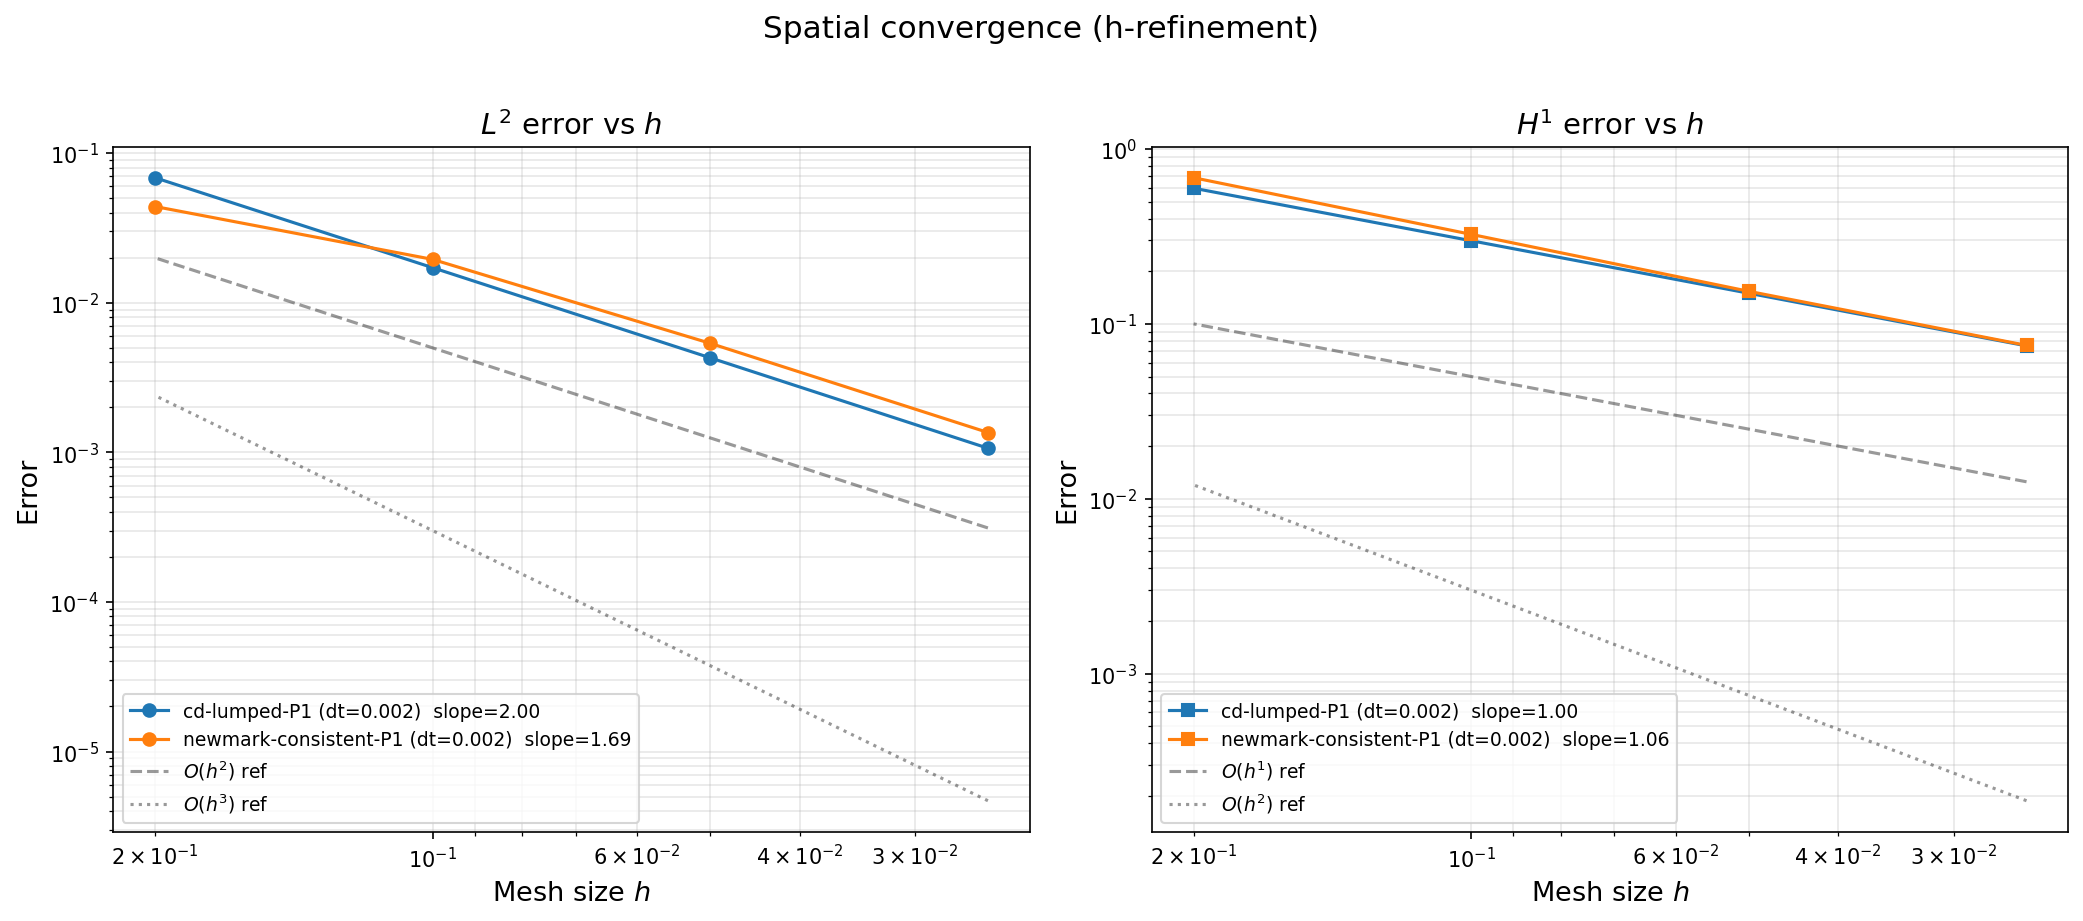
\includegraphics[width=0.82\linewidth]{convergence_h.png}

  \vspace{0.3em}
  \begin{itemize}
    \item Error decreases monotonically under mesh refinement.
    \item For smooth eigenmode benchmark, trend is close to expected
          second-order behavior in $L^2$ with P1 elements.
  \end{itemize}
\end{frame}

\begin{frame}{Temporal Convergence}
  \centering
  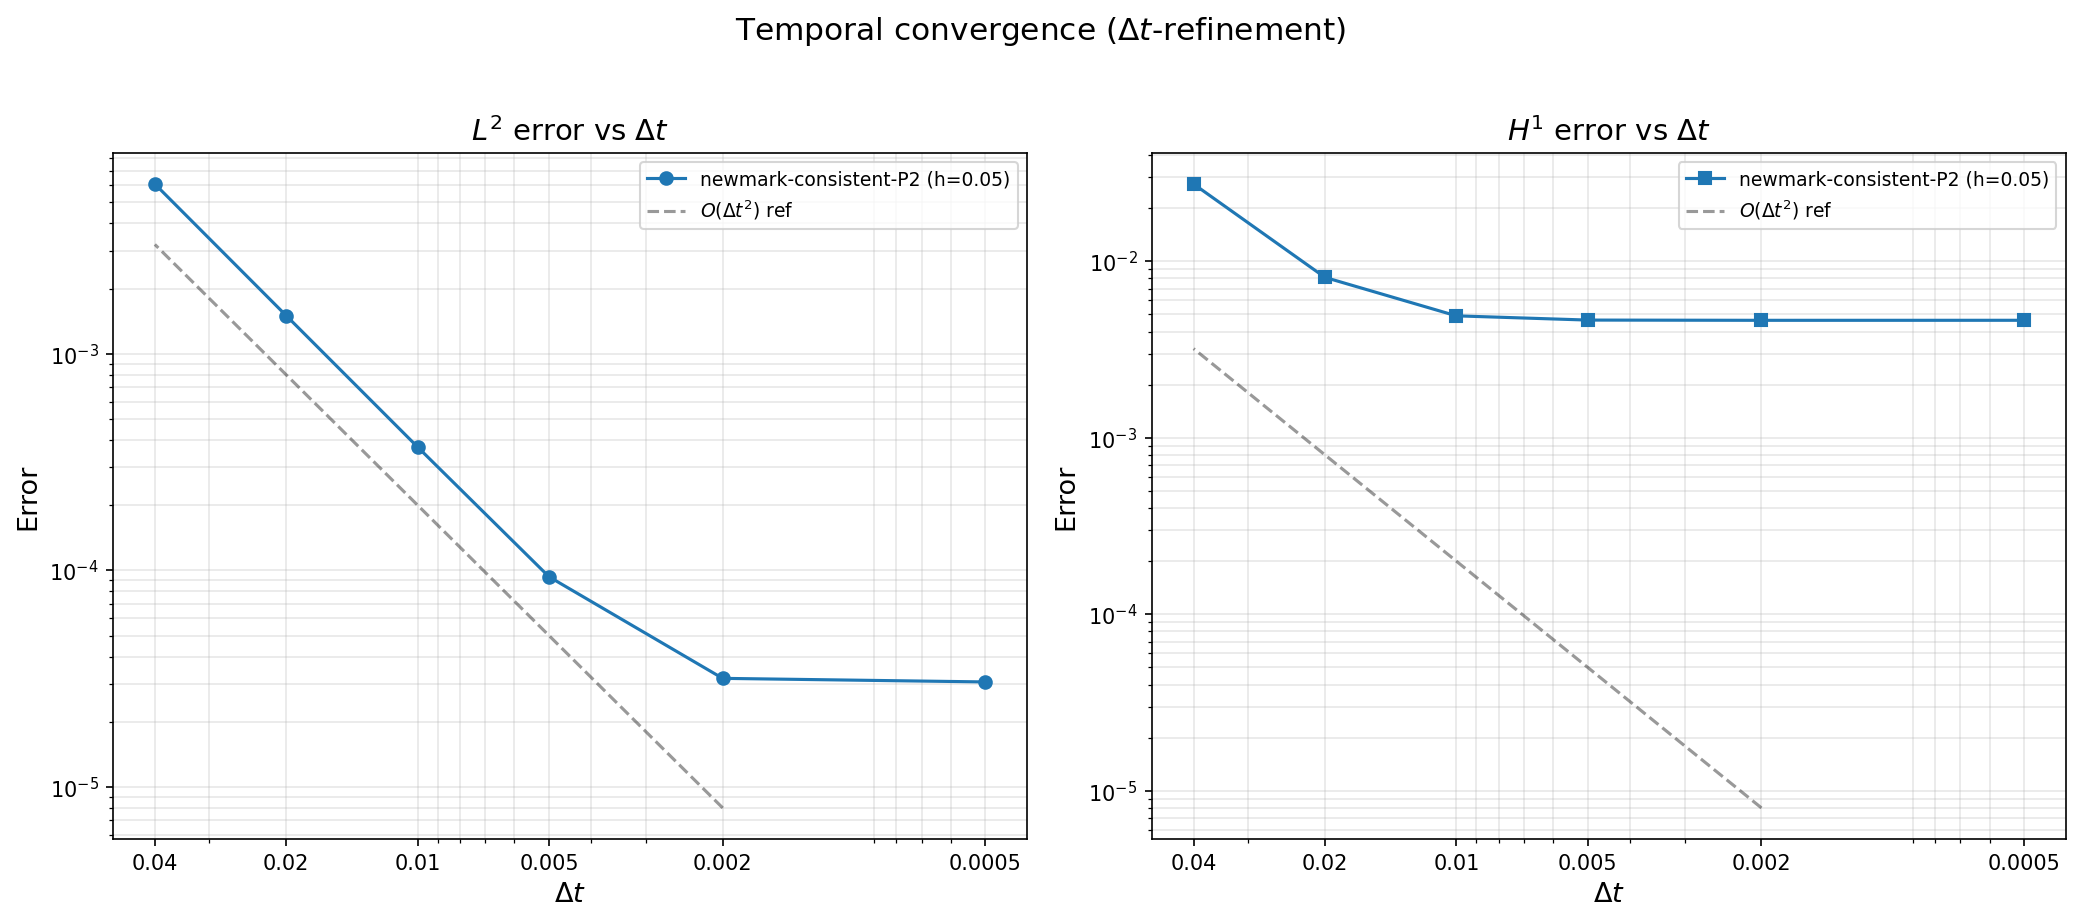
\includegraphics[width=0.78\linewidth]{convergence_dt_newmark.png}

  \vspace{0.3em}
  \begin{itemize}
    \item Reducing $\Delta t$ lowers time error until a spatial-error floor appears.
    \item Setup used here: Newmark $(h=0.05,\ P2,\ \text{consistent})$.
    \item This is consistent with
      \[
        \|u-u_h\| \lesssim C_1 h^{p+1}+C_2\Delta t^2.
      \]
  \end{itemize}
\end{frame}

\begin{frame}{Dispersion Diagnostic}
  \centering
  
\includegraphics[width=0.9\linewidth]{dispersion_relation.png}

  \vspace{0.2em}
  \begin{itemize}
    \item The ratio $\omega_h^d/\omega_{\text{exact}}$ departs from 1 at large
          normalized wavenumber.
    \item This means short waves travel with the wrong phase speed, producing
          accumulated phase error over long integrations.
  \end{itemize}
\end{frame}

\begin{frame}{Dissipation Diagnostic (Amplification Factor)}
  \begin{columns}
    \column{0.5\textwidth}
    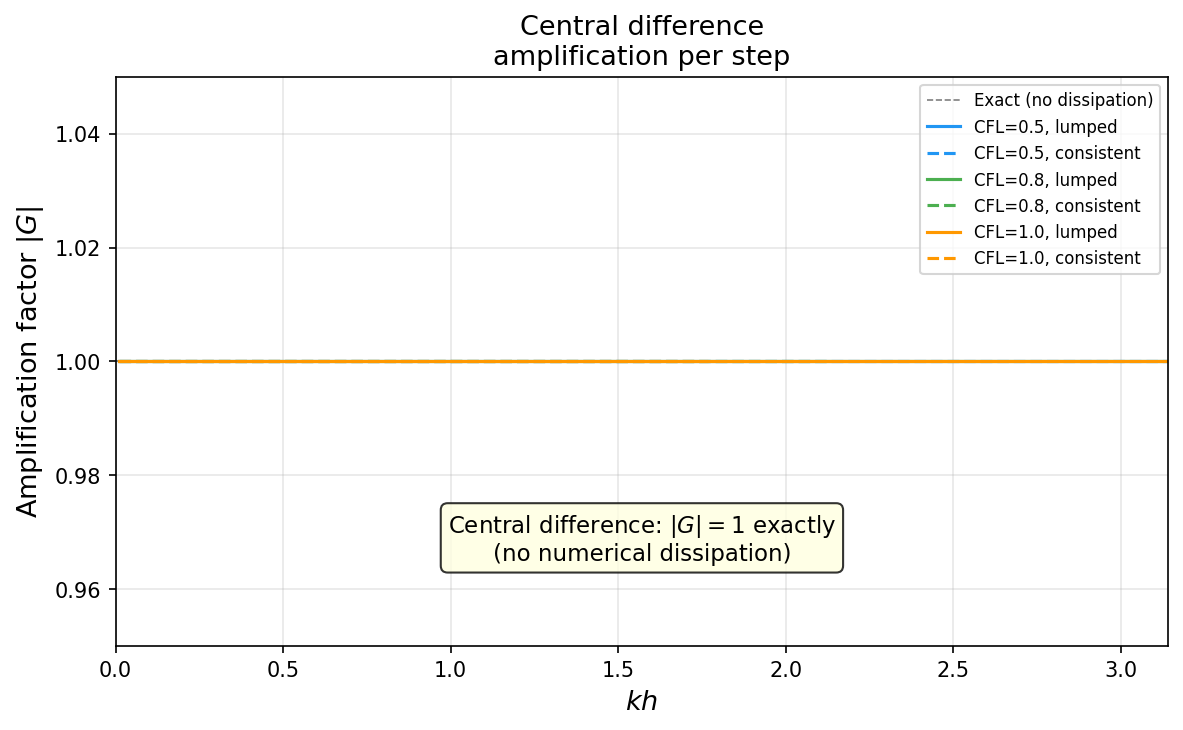
\includegraphics[width=\linewidth]{dissipation_amplification_central.png}

    \column{0.5\textwidth}
    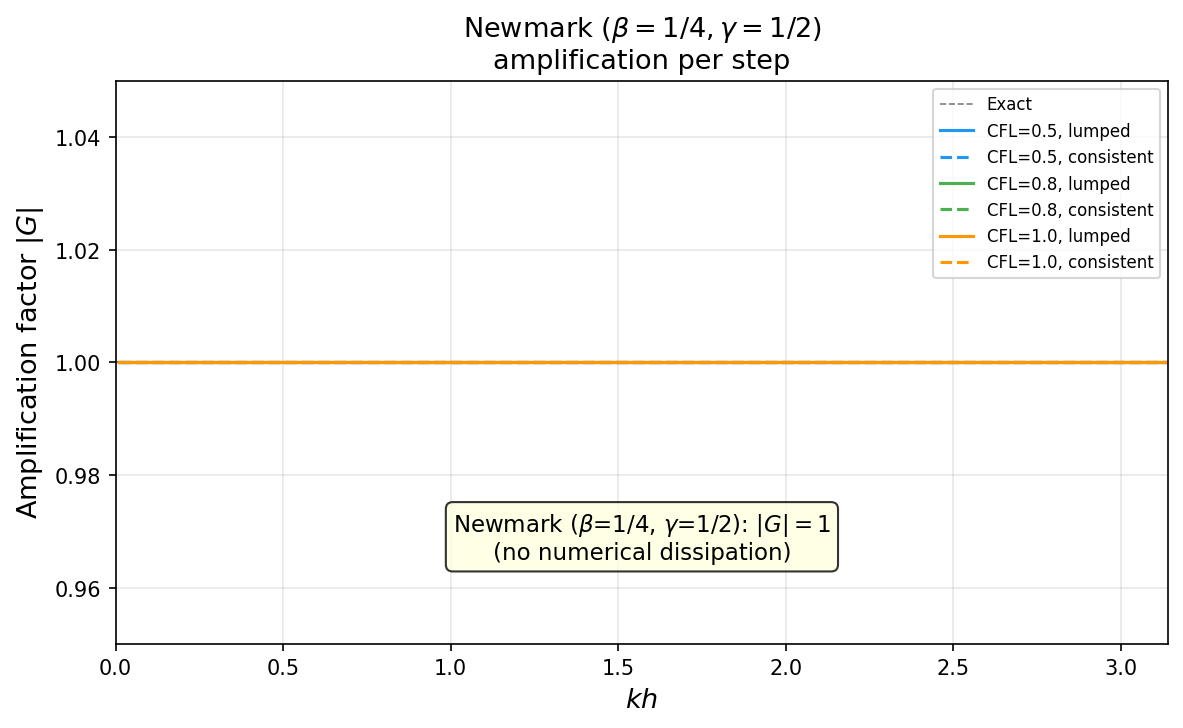
\includegraphics[width=\linewidth]{dissipation_amplification_newmark.png}
  \end{columns}

  \vspace{0.2em}
  \begin{itemize}
    \item For central difference and Newmark $(\beta,\gamma)=(1/4,1/2)$,
          curves stay close to $|G|=1$ in the stable range.
    \item Hence the dominant numerical effect is dispersion rather than strong
          artificial damping.
  \end{itemize}
\end{frame}

\begin{frame}{Energy Comparison (Same $h,\Delta t$)}
  \centering
  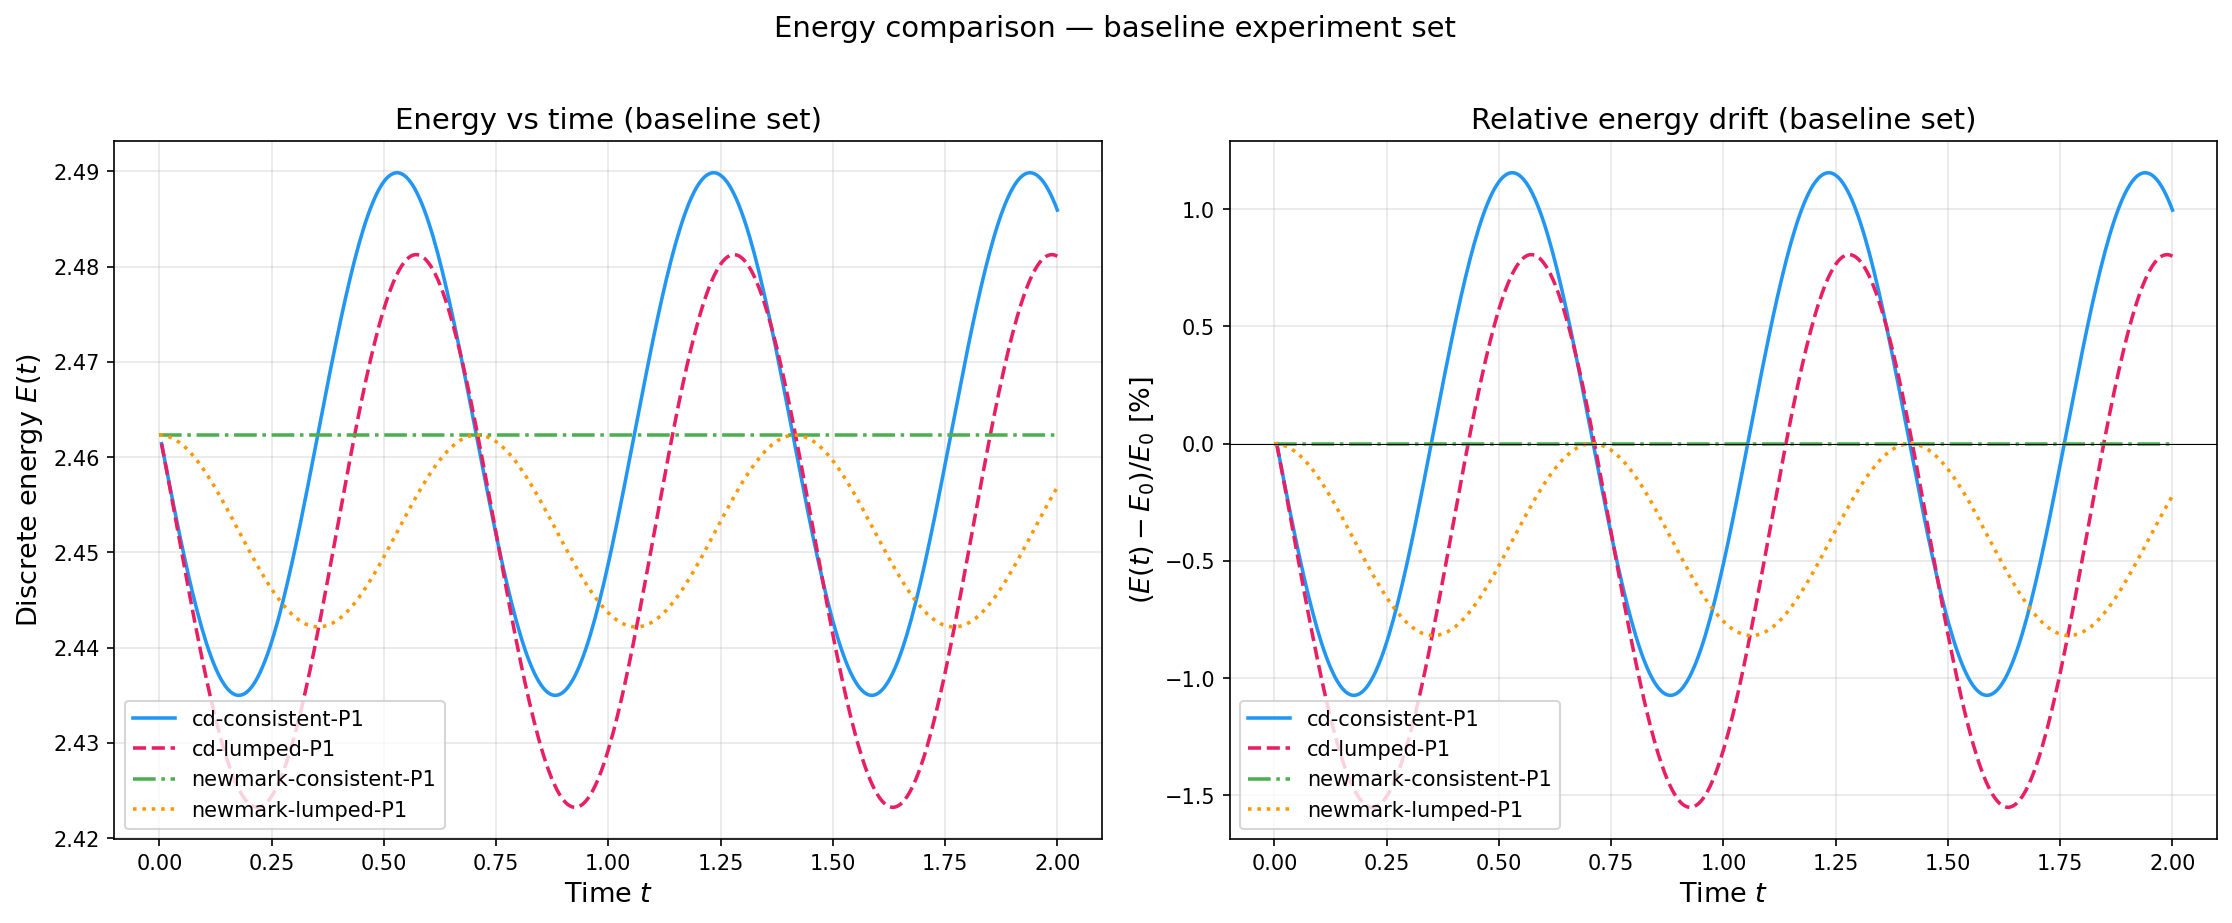
\includegraphics[width=0.72\linewidth]{energy_comparison_baseline.png}

  \vspace{0.2em}
  \begin{itemize}
    \item Central difference schemes show oscillatory energy errors.
    \item Newmark-consistent preserves energy almost exactly.
    \item Mass lumping slightly changes the energy behavior.
  \end{itemize}
   These results are consistent with our earlier conclusion that dispersion is the dominant numerical effect, while dissipation remains weak.
\end{frame}

\begin{frame}{Runtime Comparison}
  \begin{table}
    \centering
    \footnotesize
    \begin{tabular}{@{}lcccc@{}}
      \toprule
      Method + Mass & mean [s] & std [s] & median [s] & rel. \\
      \midrule
      central diff. + lumped     & 0.0154 & 0.0184 & 0.0083 & 1.00x \\
      central diff. + consistent & 0.0523 & 0.0051 & 0.0548 & 6.59x \\
      Newmark + lumped           & 0.0466 & 0.0095 & 0.0431 & 5.19x \\
      Newmark + consistent       & 0.0530 & 0.0075 & 0.0543 & 6.53x \\
      \bottomrule
    \end{tabular}
  \end{table}

  \begin{itemize}
    \item Fastest: central difference + lumped mass.
    \item Consistent mass increases cost due to repeated sparse solves.
    \item Newmark variants are costlier because of implicit linear solve each step.
  \end{itemize}
\end{frame}

\end{document}
